\documentclass[10pt]{article}
\usepackage{tikz}
\usetikzlibrary{shapes.misc}
\usepackage[margin=0cm]{geometry}
\pagestyle{empty}
\tikzstyle{every node}=[cross out, draw, red]

\begin{document}

\vspace*{\fill}
\begin{center}
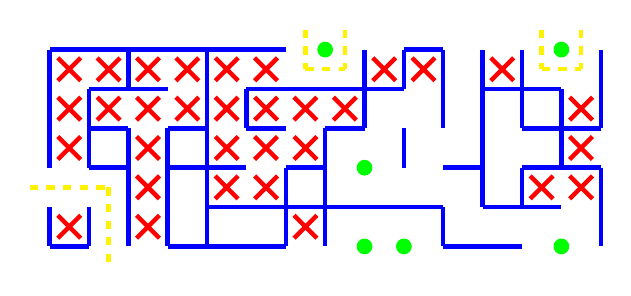
\begin{tikzpicture}[x=0.5cm, y=-0.5cm, ultra thick, blue]
% Walls
    \draw (0,0) -- (6,0);
    \draw (9,0) -- (10,0);
    \draw (1,1) -- (3,1);
    \draw (5,1) -- (9,1);
    \draw (11,1) -- (13,1);
    \draw (1,2) -- (2,2);
    \draw (3,2) -- (4,2);
    \draw (5,2) -- (6,2);
    \draw (7,2) -- (8,2);
    \draw (12,2) -- (14,2);
    \draw (1,3) -- (2,3);
    \draw (3,3) -- (5,3);
    \draw (6,3) -- (7,3);
    \draw (10,3) -- (11,3);
    \draw (12,3) -- (14,3);
    \draw (4,4) -- (10,4);
    \draw (11,4) -- (13,4);
    \draw (0,5) -- (1,5);
    \draw (3,5) -- (6,5);
    \draw (10,5) -- (12,5);
    \draw (0,0) -- (0,3);
    \draw (0,4) -- (0,5);
    \draw (1,1) -- (1,3);
    \draw (1,4) -- (1,5);
    \draw (2,0) -- (2,1);
    \draw (2,2) -- (2,5);
    \draw (3,2) -- (3,5);
    \draw (4,0) -- (4,5);
    \draw (5,1) -- (5,2);
    \draw (6,3) -- (6,5);
    \draw (7,2) -- (7,5);
    \draw (8,0) -- (8,2);
    \draw (9,0) -- (9,1);
    \draw (9,2) -- (9,3);
    \draw (10,0) -- (10,2);
    \draw (10,4) -- (10,5);
    \draw (11,0) -- (11,4);
    \draw (12,0) -- (12,2);
    \draw (12,3) -- (12,4);
    \draw (13,1) -- (13,3);
    \draw (14,0) -- (14,2);
    \draw (14,3) -- (14,5);
% Pillars
    \fill[green] (7,0) circle(0.2);
    \fill[green] (13,0) circle(0.2);
    \fill[green] (8,3) circle(0.2);
    \fill[green] (8,5) circle(0.2);
    \fill[green] (9,5) circle(0.2);
    \fill[green] (13,5) circle(0.2);
% Inner points in accessible cul-de-sacs
    \node at (0.5,0.5) {};
    \node at (1.5,0.5) {};
    \node at (2.5,0.5) {};
    \node at (3.5,0.5) {};
    \node at (4.5,0.5) {};
    \node at (5.5,0.5) {};
    \node at (8.5,0.5) {};
    \node at (9.5,0.5) {};
    \node at (11.5,0.5) {};
    \node at (0.5,1.5) {};
    \node at (1.5,1.5) {};
    \node at (2.5,1.5) {};
    \node at (3.5,1.5) {};
    \node at (4.5,1.5) {};
    \node at (5.5,1.5) {};
    \node at (6.5,1.5) {};
    \node at (7.5,1.5) {};
    \node at (13.5,1.5) {};
    \node at (0.5,2.5) {};
    \node at (2.5,2.5) {};
    \node at (4.5,2.5) {};
    \node at (5.5,2.5) {};
    \node at (6.5,2.5) {};
    \node at (13.5,2.5) {};
    \node at (2.5,3.5) {};
    \node at (4.5,3.5) {};
    \node at (5.5,3.5) {};
    \node at (12.5,3.5) {};
    \node at (13.5,3.5) {};
    \node at (0.5,4.5) {};
    \node at (2.5,4.5) {};
    \node at (6.5,4.5) {};
% Entry-exit paths without intersections
    \draw[dashed, yellow] (6.5,0.5) -- (7.5,0.5);
    \draw[dashed, yellow] (12.5,0.5) -- (13.5,0.5);
    \draw[dashed, yellow] (-0.5,3.5) -- (1.5,3.5);
    \draw[dashed, yellow] (1.5,3.5) -- (1.5,5.5);
    \draw[dashed, yellow] (6.5,-0.5) -- (6.5,0.5);
    \draw[dashed, yellow] (7.5,-0.5) -- (7.5,0.5);
    \draw[dashed, yellow] (12.5,-0.5) -- (12.5,0.5);
    \draw[dashed, yellow] (13.5,-0.5) -- (13.5,0.5);
\end{tikzpicture}
\end{center}
\vspace*{\fill}

\end{document}
